\pdfoutput=1

\def\year{2022}\relax
\documentclass[letterpaper]{article} %
\usepackage{aaai22}  %
\usepackage{times}  %
\usepackage{helvet}  %
\usepackage{courier}  %
\usepackage[hyphens]{url}  %
\usepackage{graphicx} %
\urlstyle{rm} %
\def\UrlFont{\rm}  %
\usepackage{natbib}  %
\usepackage{caption} %
\DeclareCaptionStyle{ruled}{labelfont=normalfont,labelsep=colon,strut=off} %
\frenchspacing  %
\setlength{\pdfpagewidth}{8.5in}  %
\setlength{\pdfpageheight}{11in}  %
\usepackage{algorithm}
\usepackage{algorithmic}


\usepackage[inline]{enumitem}
\usepackage{xcolor}
\usepackage{subcaption}
\usepackage{booktabs}
\usepackage{xspace}
\usepackage{multirow}

\usepackage[activate={true,nocompatibility}, kerning=true,spacing=true, stretch=10,shrink=5]{microtype}
\microtypecontext{spacing=nonfrench}
\usepackage{newfloat}
\usepackage{listings}
\lstset{%
	basicstyle={\footnotesize\ttfamily},%
	numbers=left,numberstyle=\footnotesize,xleftmargin=2em,%
	aboveskip=0pt,belowskip=0pt,%
	showstringspaces=false,tabsize=2,breaklines=true}
\floatstyle{ruled}
\newfloat{listing}{tb}{lst}{}
\floatname{listing}{Listing}

\definecolor{dkgreen}{rgb}{0,0.6,0}

\newenvironment{itemizesquish}{\begin{list}{\setcounter{enumi}{0}\labelitemi}{\setlength{\itemsep}{-0.25em}\setlength{\labelwidth}{0.5em}\setlength{\leftmargin}{\labelwidth}\addtolength{\leftmargin}{\labelsep}}}{\end{list}}

\newenvironment{enumeratesquish}{\begin{list}{\addtocounter{enumi}{1}\labelenumi}{\setlength{\itemsep}{0em}\setlength{\labelwidth}{0.5em}\setlength{\leftmargin}{\labelwidth}\addtolength{\leftmargin}{\labelsep}}}{\end{list}\setcounter{enumi}{0}}


\newcommand*\pct{\scalebox{.8}{\%}}
\newcommand{\pos}[1]{\texttt{#1}}
\newcommand{\reals}{\mathbb{R}}
\newcommand{\legalmove}{LgM\xspace}
\newcommand{\exactmove}{ExM\xspace}
\newcommand{\piecetype}{AP\xspace}




\setcounter{secnumdepth}{2}

\title{Chess as a Testbed for Language Model State Tracking}

\author{
Shubham Toshniwal\textsuperscript{\rm 1},
Sam Wiseman\textsuperscript{\rm 2},
Karen Livescu\textsuperscript{\rm 1},
Kevin Gimpel\textsuperscript{\rm 1}
}

 \affiliations{

    \textsuperscript{\rm 1}Toyota Technological Institute at Chicago\\
    \textsuperscript{\rm 2}Duke University\\
    \texttt
    {\{shtoshni, klivescu, kgimpel\}@ttic.edu, swiseman@cs.duke.edu}
}



\begin{document}

\maketitle

\begin{abstract}
Transformer language models have made tremendous strides in natural language understanding tasks.
However, the complexity of natural language makes it challenging
to ascertain how accurately these models are tracking the world state underlying the text.
Motivated by this issue, we consider the task of language modeling for the game of chess.
Unlike natural language, chess notations describe a simple, constrained, and deterministic domain.
Moreover, we observe that the appropriate choice of chess notation allows for directly probing the world state, without requiring any additional probing-related machinery.
We find that:
\begin{enumerate*}[label=(\alph*)]
	\item With enough training data, transformer language models can learn to track pieces and predict legal moves with high accuracy when trained solely on move sequences.
	\item %
	For small training sets %
	providing access to board state information during training can yield significant improvements.
	\item The success of transformer language models is dependent on access to the entire game history i.e.\ ``full attention". Approximating this full attention results in a significant performance drop.
\end{enumerate*}
	We propose this testbed as a benchmark for future work on the development and analysis of transformer language models.
\end{abstract}


%% Video grounding task %%%%%%%%%%%%%%%%%%%%%%%%%%%%%%
Temporal video grounding is a challenging task in computer vision, where the goal is to find the temporal location of starting and ending points described by a sentence query in an untrimmed video.
The task has potential for applications such as video understanding~\cite{carreira2017quo}, video summarization~\cite{ma2002user}, and video retrieval~\cite{dong2019dual}, because it can automatically extract temporal video locations of interest described by given sentences.
For temporal video grounding, a fully supervised approach has made remarkable progress~\cite{kim2021plrn,kim2022swag,gao2017tall}
but require manual annotations of temporal locations for every video-sentence pair.
These manual annotations are usually labor-intensive and noisy due to the subjectivity of annotators, which limits their scalability to real-world scenarios and makes trained models biased~\cite{yuan2021closer, zhou2021embracing}.


\begin{figure}[t!]
  \centering
  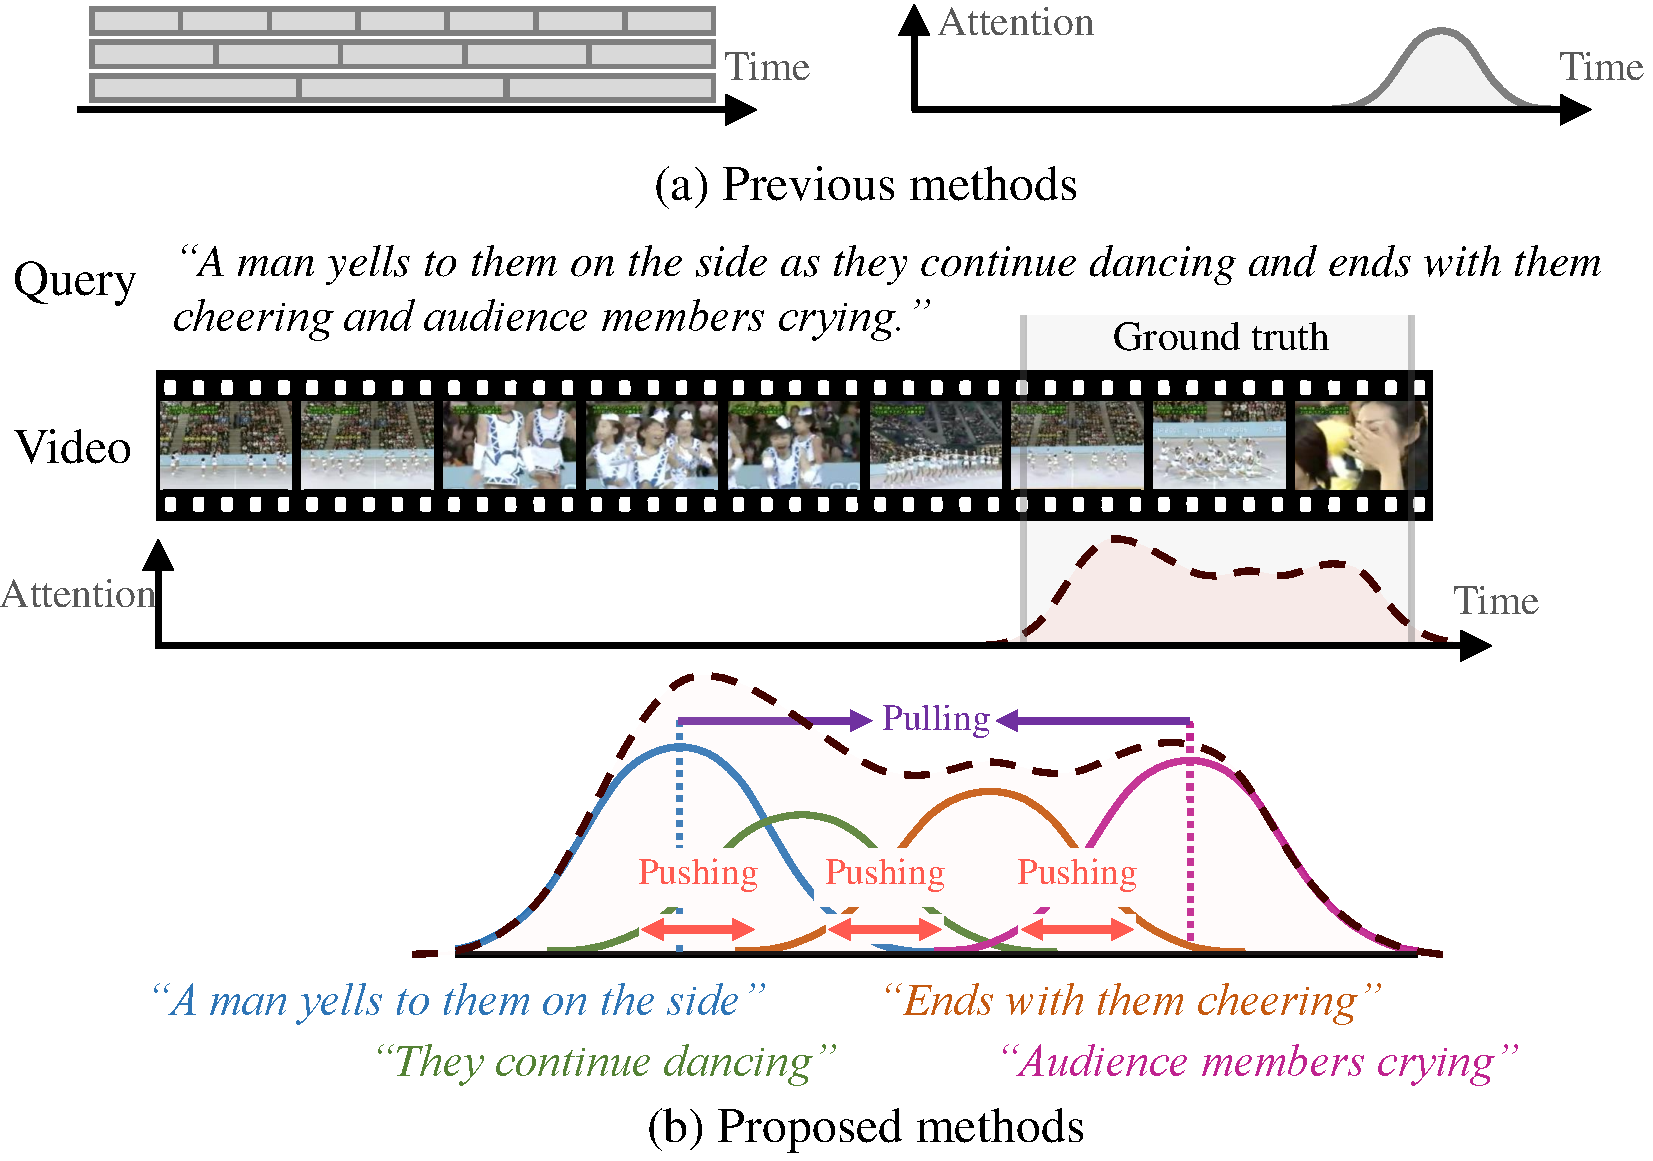
\includegraphics[width=\linewidth]{figures/0-concept-art.pdf}
  \caption{Weakly supervised temporal video grounding. (a) Previous methods use sliding windows (left) or a single Gaussian proposal (right), which has a predetermined shape. (b) The proposed method generates a Gaussian mixture proposal trained to be moderately coupled with a pull-push learning scheme to capture diverse query-relevant events.
  % Further, the proposed method leverages multiple learnable Gaussians for a negative proposal, instead of an existing rule-based one.
  }
\label{fig:concept-art}
\end{figure}

To overcome the limitation, a weakly supervised approach has been proposed to solve the temporal video grounding problem, where only video-sentence pairs are required for training. 
%% Weakly supervised video grounding methods %%%%%%%%%%%%%%%%%%%%%%%%%%%%%%
Some existing methods~\cite{huang2021cross, lin2020weakly, mithun2019weakly, tan2021logan, wang2021weakly, zhang2020counterfactual} use a sliding window strategy to generate proposals for a temporal location but use a lot of pre-defined proposals, which require heavy computation.
%and face difficulties in expressing diverse events described by the sentence query.
%% Gaussian-based methods %%%%%%%%%%%%%%%%%%%%%%%%%%%%%%
To reduce the required number of proposals, \cite{zheng2022cnm, zheng2022cpl} generate learnable Gaussian proposals. 
However, these single Gaussian proposals with a peak at its center lack the expression ability for diverse query-relevant events in a video.

To enhance the expression ability, we propose a Gaussian mixture proposal (GMP) that can depict arbitrary shapes by learning importance, centroid, and range of every Gaussian in the mixture.
% \cite{zong2018deep, lee2018simple}
Since our GMP is implemented over a temporal location, conventional feature-based learning for Gaussian mixture model~\cite{zong2018deep, lee2018simple} is not applicable to our approach.
In our special setting, our goal is to train the GMP to capture a temporal location semantically %relevant to a sentence query.
%We note that a temporal location 
relevant to a sentence query that includes diverse events coupled moderately. %coupled.
In \cref{fig:concept-art}, for instance, one sentence query includes two semantic events coupled by ``A man yells to them on the side" and ``They continue dancing".
%in the given sentence query have their own semantics but are moderately coupled to express one sentence query.

%% Proposed methods %%%%%%%%%%%%%%%%%%%%%%%%%%%%%%
To capture the %moderately 
coupled events in a query, we propose a Pull-Push Scheme (PPS) to learn a GMP whose Gaussians are moderately coupled.
Specifically, we first define a GMP with learnable parameters: importance, centroid, and range of every Gaussian in the mixture.
To learn the importance, we propose an importance weighting strategy that represents importance levels of each Gaussian mask for a query-relevant location.
To generate the GMP that represents a query-relevant location, our PPS is trained to reconstruct the sentence query from the proposal.
In our scheme, the Gaussians in one GMP should be located near a query-relevant temporal location, 
% but should not converge to an identical point to represent diverse events.
but should not be overlapped too much with others to represent diverse events.
To this end, our scheme leverages a pulling loss and a pushing loss, each of which plays an opposite role to the other to produce moderately coupled Gaussians.
The pulling loss lets the Gaussians stay close to each other by pulling the Gaussian centroids together.
% the two farthest masks together.
The pushing loss prevents the Gaussians from overlapping too much with the others by forcing the Gaussians to be less overlapped.

We verify that our scheme generates high-quality proposals that significantly improve recall rates on the Charades-STA~\cite{gao2017tall} and ActivityNet Captions~\cite{krishna2017dense} datasets.
We also demonstrate the effectiveness of each component in our scheme with extensive ablation studies.
%% Contributions %%%%%%%%%%%%%%%%%%%%%%%%%%%%%%
In summary, our contributions are as follows.
\begin{itemize}
\item We generate a Gaussian mixture proposal that represents a query-relevant temporal location by learning importance, centroid, and range of every Gaussian to enhance the expression ability of the proposal.
\item We propose a pull-push learning scheme that uses a pulling loss and a pushing loss, each of which plays an opposite role to the other to capture diverse events.
\item The proposed components are verified in-depth with extensive ablation studies and the overall scheme achieves state-of-the-art performance. 
\end{itemize}


\section{Chess Preliminaries}
\label{sec:chess}


We represent moves using Universal Chess Interface (UCI) notation, which combines the starting square and the destination square to represent a move.\footnote{For more details see \url{https://en.wikipedia.org/wiki/Universal_Chess_Interface}} 
The move in Figure~\ref{fig:move_notation} is represented as \texttt{f1b5} in UCI where \texttt{f1} indicates the starting square and \texttt{b5} denotes the ending square.
While the SAN notation is the standard choice for gameplay, we prefer UCI %
(see Appendix~\ref{sec:san} for why we pick UCI over SAN). 

For training language models, we first tokenize games represented in UCI notation using a simple regular expression based tokenizer, which considers a board square symbol such as \texttt{b1} as a single token.
This gives us a vocabulary of 77 token types, 
which includes the 64 squares, piece type symbols, and other special symbols (see Table~\ref{tab:model_vocab}).\footnote{In initial experiments we used a delimiter token to indicate move boundary. However, removing it did not degrade performance and made training faster due to reduced sequence length.}
For example, the move sequence ``\pos{e2e4 e7e5 g1f3}" is tokenized to ``\pos{e2}, \pos{e4}, \pos{e7}, \pos{e5}, \pos{g1}, \pos{f3}". We then train an autoregressive language model on these move sequences, using the standard maximum likelihood objective.

\begin{table}[t]
\centering{
\begin{tabular}{llc}
    \toprule
    Type & Examples & Count \\
    \midrule
    Square names & \pos{e4}, \pos{d1} & 64 \\
    Piece type & \pos{P}, \pos{K}, \pos{Q}, \pos{R}, \pos{B}, \pos{N} & \phantom{1}6\\
    Promoted Pawn Piece type & q, r, b, n & \phantom{1}4 \\
    Special symbols & BOS, EOS, PAD & \phantom{1}3 \\
    \midrule
    Total & & 77\\
    \bottomrule
\end{tabular}
}
\caption{Model Vocabulary}
\label{tab:model_vocab}

\end{table}

\begin{table*}
	\centering{
		\begin{tabular}{lll}
			\toprule
			Notation 		& Training 					& Inference \\\midrule
			UCI		 		& \pos{e2}, \pos{e4}, \pos{e7}, \pos{e5}, \pos{g1}, \pos{f3}     						& \pos{e2}, \pos{e4}, \pos{e7}, \pos{e5}, \pos{g1}, \pos{f3} 		\\
			UCI + RAP 15 	& \pos{e2}, \pos{e4}, \pos{P}, \pos{e7}, \pos{e5}, \pos{g1}, \pos{f3} 							& \pos{e2}, \pos{e4}, \pos{e7}, \pos{e5}, \pos{g1}, \pos{f3} 		\\
			UCI + RAP 100 	& \pos{P}, \pos{e2}, \pos{e4}, \pos{P}, \pos{e7}, \pos{e5}, \pos{N}, \pos{g1}, \pos{f3}							& \pos{e2}, \pos{e4}, \pos{e7}, \pos{e5}, \pos{g1}, \pos{f3} 		\\
			UCI + \piecetype 	& \pos{P}, \pos{e2}, \pos{e4}, \pos{P}, \pos{e7}, \pos{e5}, \pos{N}, \pos{g1}, \pos{f3}							& \pos{P}, \pos{e2}, \pos{e4}, \pos{P}, \pos{e7}, \pos{e5}, \pos{N}, \pos{g1}, \pos{f3}		\\
			\bottomrule
		\end{tabular}
	}
		\caption{Token sequences corresponding to the move sequence \pos{e2e4 e7e5 g1f3} for different notations during training and inference. Notice that regardless of the RAP probability used during training, at inference time the token sequences have no piece types.}
	\label{tab:token_seq}

\end{table*}

\section{Language Model Prompts as Board State Probes}
\label{sec:probing}
One attractive property of having a language model trained on chess games represented in UCI notation (as described in the previous section) is that the notation \textit{itself} allows us to probe the trained model's state tracking abilities. In particular, by feeding the trained language model a prefix of a game as a prompt, we can determine --- using the language model's next-token predictions --- what the model understands about the board state implied by this prefix.
For example, consider the prompt ``\pos{\underline{e2e4 e7e5 g1f3 b8c6 d2d4 h7h6} f1},''  where the underlined move sequence leads to the left board state in Figure~\ref{fig:move_notation}. A language model's next-token prediction (after consuming the prompt) can be interpreted as the ending square predicted %
for the bishop at \pos{f1}, which can be used to determine the level of board state awareness of the model. %
If, for instance, the model predicts \pos{g1}, this may indicate that the model does not recognize that the piece type at \pos{f1} is a bishop, as such a move is not possible for a bishop.
If, on the other hand, the model predicts \pos{g2}, that may indicate that the model is not aware that another piece is currently  at \pos{g2}.

\subsection{Randomly Annotated Piece type (RAP)}
\label{sec:rap_board}
While predicting the token representing the ending-square of a move given a prompt allows us to assess the model's state tracking abilities, it also to some extent conflates the model's understanding of the board state with its understanding of chess strategy. If we could easily probe for where the model thinks a piece \textit{currently} is (rather than where it is likely to end up) given a game prefix, this would allow us to more directly probe the model's state tracking abilities. 
In particular, we would like to give a language model a prompt such as ``\pos{e2e4 e7e5 g1f3 b8c6 d2d4 h7h6 \underline{N}}", where \pos{N} represents knight, and expect it to generate a valid starting position for a knight of the correct color. 
While UCI notation does not ordinarily include these piece type tokens, to allow for testing the model with such prompts, 
we propose to randomly include these piece types tokens in moves during training with some fixed probability $p$.
We refer to this strategy as ``randomly annotated piece type'' (RAP) and 
use the nomenclature ``UCI + RAP $p$'' to indicate that with $p\pct$ probability, piece type is part of the move notation during training.
Note that for $p = 0$, the notation reduces to UCI. 

When \emph{testing} with these starting square prediction prompts, we only include piece type for the prompt, not for any moves in the history.
Thus, using RAP during training allows us to probe, at test time, where the model thinks each piece is, given any game history's prefix; by simply providing the desired piece type (e.g., \pos{N}) the model outputs the predicted starting square for a piece of that type.
For example, given the prompt ``\pos{e2e4 e7e5 g1f3 b8c6 d2d4 h7h6 N}", a prediction of \pos{f3} or \pos{b1} shows that the model is aware of where the knights are.%

We also experiment with an ``oracle" variant of RAP where piece types are added both during training and testing. We refer to this notation as ``UCI + \piecetype" where AP stands for ``always piece type".
For our running example the equivalent prompt in this notation would be ``\pos{Pe2e4 Pe7e5 Ng1f3 Nb8c6 Pd2d4 Ph7h6 N}".

In terms of the language modeling training objective, addition of RAP represents a distribution change between training and inference.
Table~\ref{tab:token_seq} illustrates how the use of RAP changes the token sequence during training but not during inference.  
While there's a distribution mismatch, we hypothesize that addition of RAP can aid the model in learning to track the pieces by providing additional supervision which, in turn, can improve language modeling performance as well.  





\begin{table*}[t]
\centering
\begin{tabular}{lccc}
\toprule
Task & Prompt Token & Correct Answers (\exactmove) & Correct Answers (\legalmove) \\
\midrule
 End-Actual & \pos{f1} & \{\pos{b5}\} & \{\pos{e2, d3, c4, b5 ,a6} \} \\
End-Other & \pos{f3} & N/A & \{\pos{d2, g1, h4, g5, e5}\} \\
  \midrule
Start-Actual & \pos{B} & \{\pos{f1}\} & \{\pos{f1, c1}\} \\
Start-Other & \pos{N} & N/A & \{\pos{f3, b1}\} \\
\bottomrule
\end{tabular}
\caption{Examples of each probing task, as well as the corresponding exact move (\exactmove) and legal move (\legalmove) correct answers, are shown below. All examples assume the language model was fed the prefix \pos{e2e4 e7e5 g1f3 b8c6 d2d4 h7h6} (see Figure~\ref{fig:move_notation}), and that the actual next move was \pos{f1b5}. While there is only one valid prompt token for both End-Actual and Start-Actual tasks, there are many valid prompt tokens for the other tasks, and we show just one possibility for each. Start-tasks (bottom sub-table) assume the model was trained on games described in UCI+RAP notation.}
\label{tab:tasks}

\end{table*}

\subsection{Board State Probing Tasks}
\label{sec:cloze}
In this subsection we describe the probing tasks introduced above more concretely. %
In each probing task we feed the model a prefix of a game followed by a single prompt token, and the model is evaluated based on the highest probability next-token under the model given this context. We show an example of each probing task in Table~\ref{tab:tasks} (which we further describe below), assuming the model has been fed the move sequence prefix \pos{e2e4 e7e5 g1f3 b8c6 d2d4 h7h6}, %
which is visualized as the left board in Figure~\ref{fig:move_notation}. The actual next move played in the game is \pos{f1b5}, which takes the white bishop at square \pos{f1} to square \pos{b5}, as shown in the right board of Figure~\ref{fig:move_notation}. 


\subsection{Ending Square Tasks}
In this set of tasks, the model is given a game prefix and prompted with the starting square of the next move (\pos{f1} in the example of Table~\ref{tab:tasks}). The model's next-token prediction represents its prediction for the ending square of this move,
which
tests the model's ability to track the board state and follow
the rules of chess,
as well as strategic awareness.\footnote{Strategic capabilities of a chess language model are strongly tied to the quality of training games.}  We consider two task variants: %
\begin{enumerate}
	\item \textbf{End-Actual}: Given a move sequence prefix, the model is prompted with the starting square of the actual piece moved next in the game. %
	\item \textbf{End-Other}: Given a move sequence prefix, the model is prompted with the starting square of any piece on the board that can be legally moved according to the rules of chess. 
\end{enumerate}
We evaluate End-Actual predictions in terms of both exact move (\exactmove) accuracy (whether the model predicted the true ending square, \pos{b5} in our running example) and legal move (\legalmove) accuracy (whether the model predicted a legal ending square for the piece starting at the square in the prompt). 
For \legalmove evaluation, we also calculate the R-Precision which is the Precision@R where R is the total number of legal ending squares~\cite{ir-book}. In our running example, there are 5 legal ending squares, and R-Precision will be calculated for the model's top-5 predictions.
\exactmove accuracy evaluation is similar to the typical evaluation of language models on natural language data, while \legalmove is less stringent and focuses on testing just the model's understanding of chess rules and the board state. Note that for End-Other, only \legalmove evaluation is available. See Table~\ref{tab:tasks} for examples.


\subsection{Starting Square Tasks}
In this category of task, the model is again given a game prefix, but prompted with just the piece type of the next move, such as \pos{B} for bishop in the example in Table~\ref{tab:tasks}. The model's next-token prediction thus represents its prediction for where the prompted piece type currently is on the board. This task tests the model's ability to track pieces.\footnote{In certain cases, this task also tests understanding of chess rules. For example, in Figure~\ref{fig:move_notation} only the rook at \pos{h1} can be moved.}
Note that only models which have seen piece types during training, i.e.\ ``UCI + RAP'' models, can actually be tested on this task.
Also, no piece types are used in the game prefix. %
We again have two variants of this task:
\begin{enumerate}
	\item \textbf{Start-Actual}: Given a move sequence prefix, the model is prompted with the piece type of the actual piece moved next in the game. 
	\item \textbf{Start-Other}: Given a move sequence prefix, the model is prompted with the piece type of any piece on the board that can be legally moved according to the rules of chess. %
\end{enumerate}
We again evaluate Start-Actual %
both in terms of \exactmove accuracy (whether the model predicts the starting square of the piece actually moved next in the game), as well as in terms of \legalmove accuracy (whether the model predicts the starting square of a legally movable piece of the given piece type) and \legalmove R-Precision (precision of the model's top-R predictions with respect to all of the R starting squares of legally movable pieces of the given piece type). For Start-Other, only \legalmove evaluation is applicable; see Table~\ref{tab:tasks} for examples.


\section{Experimental Setup}
\label{sec:setup}

\paragraph{Data}
We use the Millionbase dataset which is freely available and has close to 2.9 million quality chess games.\footnote{Download link available at \url{https://rebel13.nl/rebel13/rebel\%2013.html}}
After filtering out duplicate games, games with
fewer than 10 moves, and games with
more than 150 moves (for the complete game to fit into one transformer window), we are left with around 2.5 million games.
From this filtered set we randomly select 200K games for training, 15K games each for dev and test, and another 50K games to create board state probing evaluation sets described in Section~\ref{sec:cloze}.
The dev and test sets are used for perplexity evaluations. 
The dev set perplexity is used for choosing hyperparameters.
From the 200K training set, we create subsets of size 15K and 50K which we refer to as ``Train-S'' and ``Train-M'', while the full training set is referred to as ``Train-L''.
For detailed statistics, see Table~\ref{tab:data_stats} in Appendix.
All the data processing steps requiring chess knowledge, including parsing chess databases, are carried out using python-chess~\citep{python-chess}.

To create the board state probing evaluation sets, we use the 50K games reserved for this task. %
We only consider prompts for non-pawn pieces since the dynamics of pawns are fairly limited.
We ensure that the game prefixes selected are never seen in the training data.
The final evaluation set consists of 1000 instances with prefix length (in number of moves) in the range $51 \le l \le 100$.





\begin{figure*}
	\begin{minipage}{\textwidth}
		\begin{minipage}[b]{0.48\textwidth}
			\centering
			\begin{tabular}{llcc}
				\toprule
				Training Set & Model   & Dev set & Test set \\
				\midrule
				\multirow{2}{*}{Train-S} 
				& UCI 				& 23.6 & 23.6\\
				& UCI + RAP 		& 15.9 & 15.9\\
				& UCI + \piecetype 	& 16.1 & 16.2 \\
				\midrule
				\multirow{2}{*}{Train-M} 
				& UCI 				& 11.6 & 11.6\\
				& UCI + RAP 		& 10.4 & 10.4\\
				& UCI + \piecetype 	& 10.1 & 10.0 \\
				\midrule
				\multirow{2}{*}{Train-L} 
				& UCI 				& \phantom{1}7.7 & \phantom{1}7.7\\
				& UCI + RAP 		& \phantom{1}7.4 & \phantom{1}7.4\\
				& UCI + \piecetype 	& \phantom{1}7.2 & \phantom{1}7.2 \\
				\bottomrule
				
			\end{tabular}
			\captionof{table}{Canonical validation and test set perplexity. By canonical we mean that one move, say \pos{f1b5}, counts as one token.}
			\label{tab:perplexity}
		\end{minipage}
		\hfill
		\begin{minipage}[b]{0.48\textwidth}
			\centering
			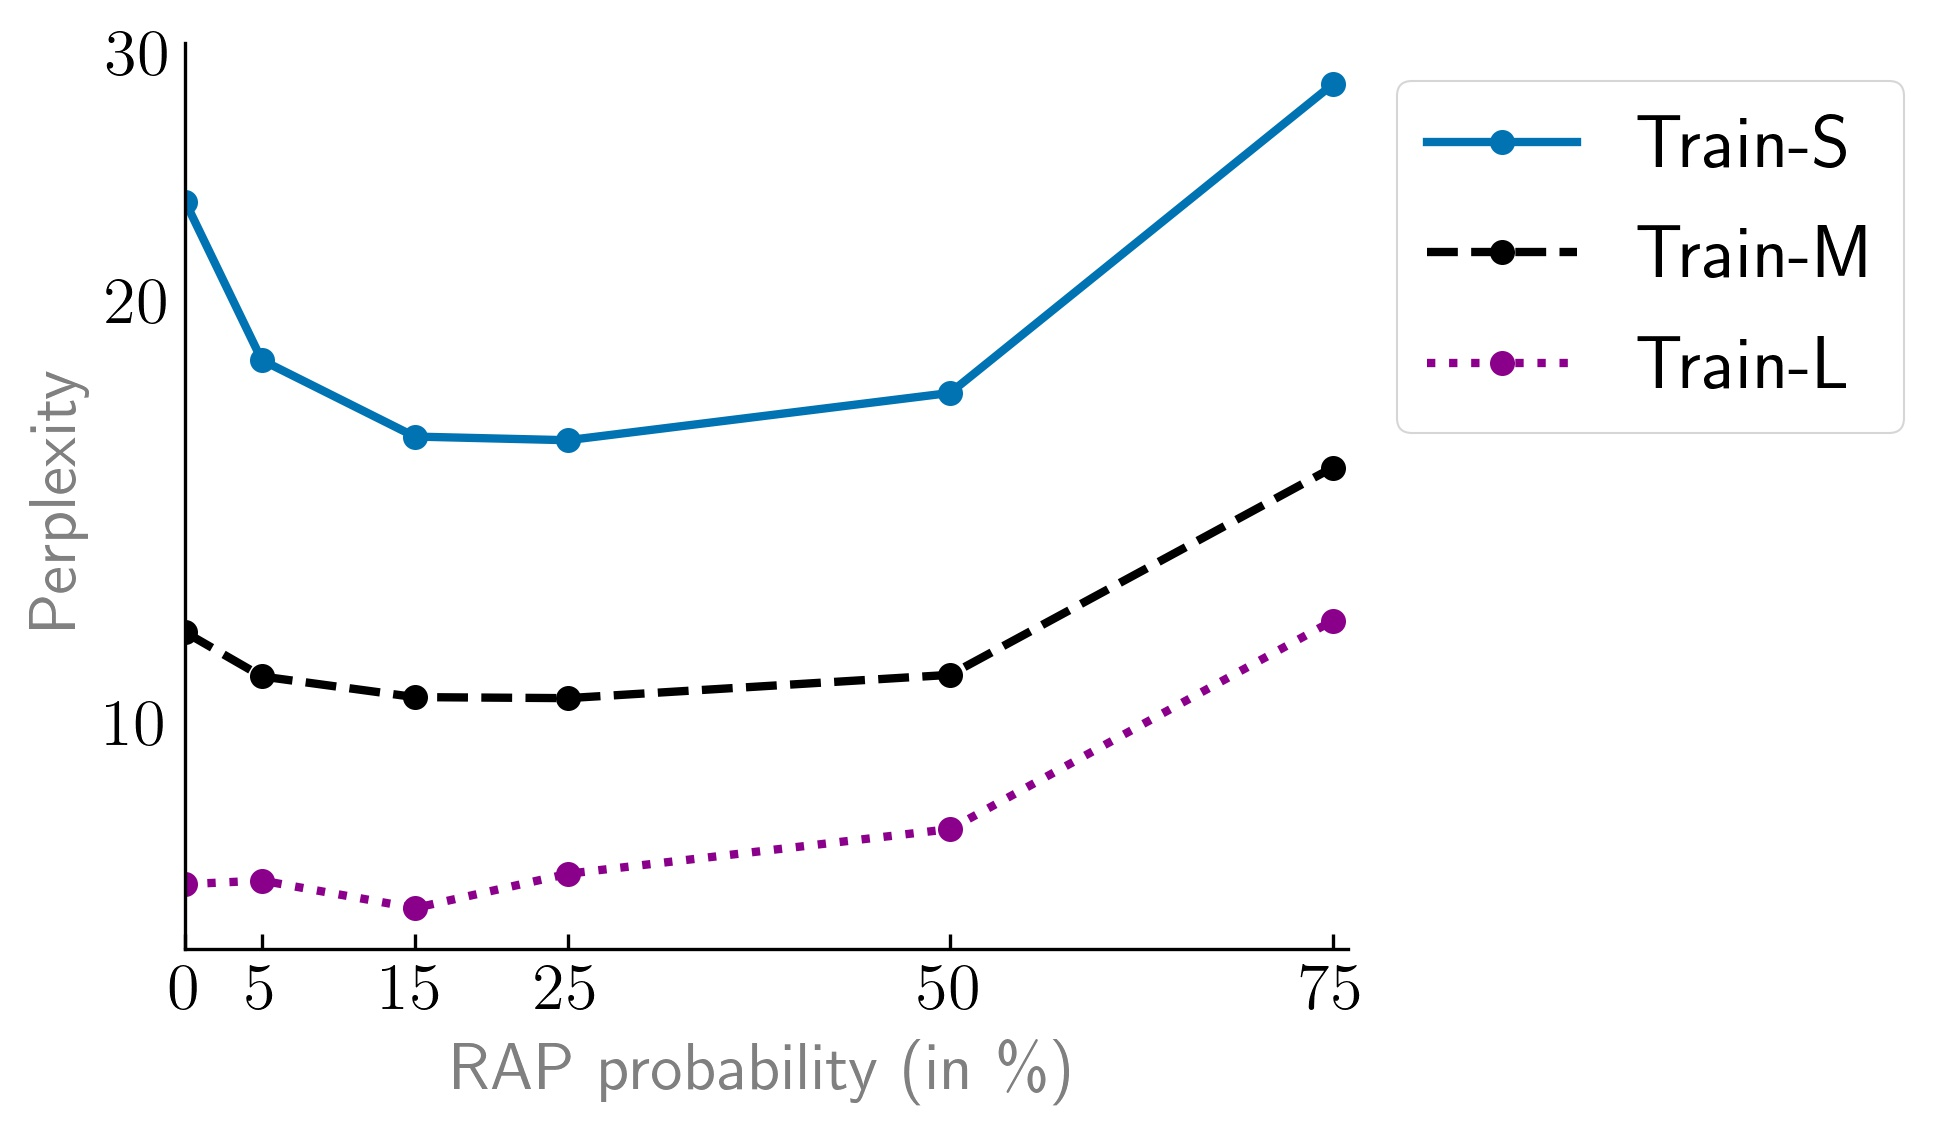
\includegraphics[width=\textwidth]{figures/rap_effect.jpg}
			\captionof{figure}{Validation set perplexities as a function of RAP probabilities for the different training set sizes. RAP $0$ %
				is %
				the standard UCI notation. 
				RAP $100$ is not shown as perplexities are too high. }
			\label{fig:rap_vals}
		\end{minipage}
	\end{minipage}
\end{figure*}

\paragraph{Model Details}
We use the GPT2-small architecture for our base language model \citep{vaswani2017attention,radford2019language}.
GPT2-small is a 12-layer transformer model with 12 attention heads and an embedding size of 768 dimensions.
The context size of the model is limited to 512, which is sufficient to cover the longest game in our training set.
Note that we only borrow the model architecture; the models themselves are \emph{trained from scratch}.
\footnote{Colab notebook to play chess against the base language model \url{https://github.com/shtoshni/learning-chess-blindfolded/blob/master/GPT2_Chess_Model.ipynb}}


For the UCI + RAP $p$ models, we tune over $p \in \{5, 15, 25, 50, 75, 100\}$ based on %
perplexity on the validation set.
Note that for perplexity evaluation, logits corresponding to piece type tokens are masked out since piece type tokens are only available during training.
We find that $p=25$ performs the best for Train-S and Train-M, while $p=15$ is best for Train-L (Figure~\ref{fig:rap_vals}). %
Larger values of $p$ lead to greater mismatch between training and inference, while smaller values likely do not provide enough training signal.

We also experiment with other transformer and non-transformer models in Section~\ref{sec:other_models}.
Among the transformer models, we experiment with two ``approximate" attention models (i.e., models which approximate the full attention of vanilla transformer models), namely, Reformer \cite{kitaev2020reformer} and Performer \cite{choromanski2021rethinking}.  
We set the number of layers and attention heads to 12 for both 
architectures, as in GPT2-small.
We also train LSTM language models with and without RAP. 
For details on hyperparameters and tuning, see Appendix~\ref{sec:hyperparams}.


\paragraph{Training Details}
Models are trained for 10 epochs with a batch size of 60. Validation is performed %
 at the end of every epoch and training stops whenever the validation loss starts increasing.
For optimization we use Adam \citep{kingma2014adam} with learning rate of $5\times10^{-4}$ and L2 weight decay of $0.01$.
The learning rate is warmed up linearly over the first 10\% of training followed by a linear decay.
To accelerate training, we use mixed precision training~\citep{micikevicius2018mixed}. %
All experiments are carried out using the PyTorch Lightning framework %
built on top of PyTorch \citep{falcon2019pytorch, pytorch}.
We use the transformers library \citep{Wolf2019HuggingFacesTS} for all models\footnote{Reformer implementation in \pos{transformers} library is still a work in progress. The presented results are with the 4.2.2 version.} %
except for the Performer model %
for which we use a popular unofficial implementation.
\footnote{\url{https://github.com/lucidrains/performer-pytorch}}









\section{Results}
We first present language modeling results, where we show significant 
improvements with the addition of RAP (Section~\ref{sec:perplexity_res}). 
Next, we show results on the board state probing tasks for the base language model, where we demonstrate that the 
model trained on the large training set can learn to track pieces and predict legal moves with high accuracy (Section~\ref{sec:state_tracking_res}).
Finally, we present results on the probing task 
with approximate attention transformer architectures and LSTMs,  where we show a performance drop in comparison to the base model with full attention (Section~\ref{sec:other_models}).



\subsection{Language Modeling}
\label{sec:perplexity_res}
Table~\ref{tab:perplexity} presents the perplexity results on the validation and test sets.  
Figure \ref{fig:rap_vals} plots the validation set perplexities as a function of RAP probability for different training set sizes. 
The addition of RAP and \piecetype leads to a decrease in perplexity for all training sizes, particularly for small training sets.
For small training sets, RAP probabilities as high as 50\% can improve the validation perplexity, but for larger training sets, lower RAP probabilities are preferred. 
The reductions in perplexity for RAP are surprising given that the extra tokens added via RAP are not present in the validation and test sets, and thus there is a data distribution shift. %
Models trained with UCI + \piecetype achieve the lowest perplexities on larger training sets. 
Both RAP and \piecetype aid the model in piece tracking, as we will see in later results, and in the case of chess this can significantly improve the language modeling results as well.
Note that for calculating the perplexity of UCI + RAP models, we mask out the logits corresponding to piece type tokens since they are never present during inference. 



\subsection{Board State Tracking}
\label{sec:state_tracking_res}
Tables~\ref{tab:results-starting} and~\ref{tab:results-ending} show results when predicting starting squares and ending squares, respectively. 
There are several observations to note. First,  \textbf{transformers can learn to identify where pieces are located}.
This is shown by the \legalmove accuracies in Table~\ref{tab:results-starting}.
UCI + RAP can predict legal starting positions with perfect accuracy and R-Precision. 
However, this capability requires Train-L, and the accuracy drops to 91.3\% for Train-S. 
The gap between UCI + RAP and its ``oracle" counterpart, UCI + \piecetype, also reduces with an increase in training set size with UCI + RAP achieving parity for Train-L.
When asked to identify the location of a piece other than the one selected to be moved next, this accuracy drops only slightly to 99.6\%. 
Typically, the piece location tracking is slightly better for the piece type that is actually moved 
than for other piece types.

The difference between the location of the piece in the exact move (\exactmove) and the location of either piece of the given type (\legalmove) is substantial, at more than 8\% absolute.  
However, this difference relates to chess strategy rather than board state tracking. 


\begin{table}[t]
	\setlength\tabcolsep{4pt}
	\centering{
		\begin{tabular}{llccccc}
			\toprule
			&  Notation 	&  \multicolumn{4}{c}{\legalmove} & \exactmove\\
			
			&  &  \multicolumn{2}{c}{Actual} &   \multicolumn{2}{c}{Other} &  \\
			&  &  Acc. & R-Prec. & Acc. & R-Prec. & Acc.\\
			\midrule
			\multirow{2}{*}{S} 	& UCI + RAP& \phantom{1}91.3 & \phantom{1}90.2 & \phantom{1}89.3 & \phantom{1}89.2  & 78.8 \\
			& UCI + AP & \phantom{1}99.2 & \phantom{1}99.1 & \phantom{1}98.8 & \phantom{1}98.8  & 86.9 \\
			\midrule
			\multirow{2}{*}{M} 	& UCI + RAP & \phantom{1}98.2 & \phantom{1}98.0 & \phantom{1}98.6 & \phantom{1}98.7  & 88.0 \\
			& UCI + AP  & \phantom{1}99.9 & \phantom{1}99.8 & 100.0 & 100.0  & 90.2 \\
			\midrule
			\multirow{2}{*}{L} 	& UCI + RAP& 100.0 & 100.0 & \phantom{1}99.6 & \phantom{1}99.5  & 91.8 \\
			& UCI + AP & \phantom{1}99.9 & \phantom{1}99.9 & \phantom{1}99.7 & \phantom{1}99.7  & 91.1 \\
			\midrule
			\multicolumn{2}{l}{Random Legal}  & - & - & - & - & 86.0\\
			\bottomrule
		\end{tabular}
		
	\caption{Accuracies and R-Precisions (\%) for predicting starting squares (``Start-Actual'' and ``Start-Other'' tasks). S, M, L in the first column refer to the training set sizes. 
	}
	\label{tab:results-starting}
	
}
\end{table}
\begin{table}
	\setlength\tabcolsep{4pt}
	\centering{
		\begin{tabular}{llccccc}
			\toprule
			&  Notation 	&  \multicolumn{4}{c}{\legalmove} & \exactmove\\
			
			&  &  \multicolumn{2}{c}{Actual} &   \multicolumn{2}{c}{Other} &  \\
			&  &  Acc. & R-Prec. & Acc. & R-Prec. & Acc.\\
			\midrule
			\multirow{3}{*}{S}
			& UCI  				&  74.0 & 61.1 & 65.5 & 57.7  & 26.7 \\
			& UCI + RAP  		&  88.4 & 75.5 & 80.4 & 72.1  & 33.3  \\
			& UCI + \piecetype 	&  87.0 & 77.0 & 78.8 & 72.3  & 36.1   \\
			\midrule
			\multirow{3}{*}{M}
			& UCI  				&  92.9 & 80.6 & 85.8 & 78.5  & 42.2  \\
			& UCI + RAP  		&  94.9 & 82.2 & 87.9 & 78.0  & 45.9  \\
			& UCI + \piecetype 	&  94.7 & 82.4 & 88.3 & 79.1  & 47.3   \\ 
			\midrule
			\multirow{3}{*}{L}
			& UCI  				&  97.7 & 85.6 & 91.9 & 83.8  & 52.0   \\
			& UCI + RAP  		&  97.0 & 86.1 & 93.1 & 83.9  & 54.7  \\
			& UCI + \piecetype 	&  98.2 & 87.3 & 95.2 & 86.3  & 56.7  \\
			\midrule
			\multicolumn{2}{l}{Random Legal} & - & - & - & - & 19.6 \\
			\bottomrule
			
		\end{tabular}
	\caption{Accuracies and R-Precisions (\%) for predicting ending squares (``End-Actual'' and ``End-Other'' tasks). S, M, L in the first column refer to the training set sizes.
	}
	\label{tab:results-ending}
	
	}
\end{table}


Second, \textbf{transformers can learn to predict legal moves}.
This is shown by the \legalmove accuracies in  Table~\ref{tab:results-ending}, for which both UCI and UCI + RAP exceed 97\% accuracy. 
However, while the top predictions of the models have high accuracy, their ability to predict all legal moves is significantly lower, with R-precision of about 85\%. 
This is to be expected, since the model is trained on only actual games, where the emphasis is on ``meaningful" moves rather than any legal move. 
Due to similar reasons, there's a significant drop in performance when predicting ending squares for starting squares other than the one in the actual game. 
	The ``other" starting square would, by design, have legal continuations, but lack any ``meaningful" ones 	(see examples in Appendix \ref{sec:app_error_analysis}).



We find consistent gains in almost all metrics with the addition of RAP during training, with the gains being particularly impressive for small training sets. Thus, not only are the transformers robust to distribution shift due to RAP (available only during training), they are in fact able to utilize this additional information. Error analysis of illegal predictions shows that the addition of RAP improves piece tracking related errors (Appendix~\ref{sec:error_analysis}).  

The relatively low ExM accuracies of the models can be attributed to the inherent difficulty of the task.   
Randomly selecting an ending square from all legal ending squares 
has an accuracy of only around 20\%, implying that on average there are roughly 5 legal choices, which might explain the difficulty of the task.  

\begin{table}[t]
\centering{
		\setlength\tabcolsep{3.1pt}
		\begin{tabular}{llccccc}
			\toprule
			&  Model 	&  \multicolumn{4}{c}{\legalmove} & \exactmove\\
			
			&  &  \multicolumn{2}{c}{Actual} &   \multicolumn{2}{c}{Other} &  \\
			&  &  Acc. & R-Prec. & Acc. & R-Prec. & Acc.\\
			\midrule
			\multirow{6}{*}{S}
			& GPT2  				&  74.0 & 61.1 & 65.5 & 57.7  & 26.7  \\
			& GPT2 ($w=50$)    			& 69.5 & 57.4 & 60.4 & 53.2  & 23.1  \\
			
			& Reformer				&  71.0 & 57.2 & 61.5 & 53.5  & 24.8 \\
			& Performer				&  65.4 & 54.3 & 57.9 & 49.5  & 20.5  \\
			& LSTM 					&  60.2 & 51.0 & 52.5 & 46.4  & 20.9  \\
			& LSTM + RAP 			&  59.5 & 50.5 & 52.4 & 46.0  & 21.9 \\
			
			\midrule
			\multirow{6}{*}{M}
			& GPT2  				&  92.9 & 80.6 & 85.8 & 78.5  & 42.2   	\\
			& GPT2 ($w=50$)  			&  86.0 & 74.9 & 80.9 & 71.3  & 35.8  	\\
			& Reformer 				&  86.4 & 73.2 & 76.6 & 68.6  & 32.4 	\\
			& Performer 			&  89.2 & 76.3 & 80.5 & 71.5  & 36.0   	\\
			& LSTM  				&  73.8 & 61.6 & 67.2 & 59.8  & 32.0   	\\
			& LSTM + RAP 			&  77.5 & 64.9 & 69.7 & 61.7  & 32.1  	\\ 
			\midrule
			\multirow{6}{*}{L}
			& GPT2  				&  97.7 & 85.6 & 91.9 & 83.8  & 52.0  	\\
			& GPT2 ($w=50$)    		&  95.8 & 84.5 & 90.5 & 82.7  & 51.6  	\\
			& Reformer 				&  88.0 & 74.9 & 77.0 & 68.1  & 33.5 	\\
			& Performer				&  95.8 & 84.5 & 90.5 & 82.7  & 51.6  	\\
			
			& LSTM  				&  93.4 & 79.5 & 86.1 & 76.0  & 45.2  	\\
			& LSTM + RAP 			&  92.8 & 80.4 & 87.3 & 77.1  & 46.0	\\
			\bottomrule
			
		\end{tabular}
		
	\caption{Accuracy and R-Precision (\%) for predicting ending squares (``End-Actual'' and ``End-Other'' tasks)  with varying attention window sizes. 
		LSTM + RAP refers to LSTM  trained with UCI + RAP.
	}
	\label{tab:results-ending-window}
	
	}
\end{table}


\subsection{Compressing the Game History}
\label{sec:other_models}
The base transformer language model, based on GPT2, attends to the entire history (i.e., it uses ``full attention"), which results in complexity quadratic in the length of the sequence. We might wonder whether attending to this entire history is necessary for the impressive state tracking performance observed in the %
previous section.
We accordingly 
explore models that do not attend to the entire history in Table \ref{tab:results-ending-window}. %

We first experiment with a variant of the GPT2 model that limits its attention to a window of only the 50 most recent tokens (``GPT2 $(w=50)$''). In Table \ref{tab:results-ending-window} we see worse performance for this model across data sizes, but especially for small- and medium-sized datasets. 

In Table~\ref{tab:results-ending-window} we also consider a language model based on the LSTM~\citep{hochreiter1997long}, which considers only its current hidden state and cell state in making its predictions, and does not explicitly attend to the history. %
Here we find an even more significant drop in performance, in all settings. (Interestingly, we also find that training LSTM language models on sequences with RAP improves performance, but only for larger training sets; transformer language models generally improve when trained with RAP data). 

The results of GPT2 $(w = 50)$ and of the LSTM language model suggest that attending to the full game history is, unsurprisingly, useful for board state tracking in chess. This finding further suggests that the task of board state tracking in chess can serve as an excellent testbed for recently proposed transformer variants~\citep[\textit{inter alia}]{kitaev2020reformer,katharopoulos20,choromanski2021rethinking} that attempt to make use of long histories or contexts, but \textit{without} incurring a quadratic runtime. 



\subsubsection{Approximate Attention Transformers}
\label{sec:limited_history}

We experiment with the recently proposed Reformer~\cite{kitaev2020reformer} and Performer~\cite{choromanski2021rethinking} architectures. Reformer replaces the ``full attention" with attention based on locality-sensitive hashing, while Performer approximates the ``full attention" with random features.\footnote{In practice, these models often use a combination of the proposed approximate global attention and simple local attention (for details see Appendix~\ref{sec:hyperparams}).}

The results, in Table~\ref{tab:results-ending-window}, suggest that the Performer generally outperforms the Reformer, except in the small dataset-setting. Furthermore, we find that neither of these architectures significantly outperforms the GPT2 $(w = 50)$ baseline, except for Performer in the medium-sized data setting. 
These models do, however, typically outperform the LSTM models. 
These results demonstrate the challenge of modeling chess with an approximate attention. 
We hope that future work will use this task as a way of benchmarking more efficient transformer architectures. %














\section{Related Work}
\paragraph{Simulated Worlds.} %
There have been several prior efforts in relating simulated worlds to natural language. 
The bAbI framework simulates a world modeled via templates to generate question answering tasks \citep{weston2015aicomplete}. 
The recent TextWorld framework facilitates generating, training, and evaluating interactive text-based games \citep{cote18textworld}. 
\citet{hermann17grounded} and \citet{hill17understanding} develop and use 3D world simulations for learning grounded language.
These efforts are similar to our work in the sense that the true world state is, by construction, available, but our setup differs in that it provides a natural way of probing the state tracking of a model trained with an LM objective.




\paragraph{Cloze Tasks for Natural Language Models.}
There has been a great deal of work on cloze tasks for evaluating natural language models~\citep{hermann2015cnn, hill2016cbt}. 
These tasks range from testing general text understanding~\citep{paperno-etal-2016-lambada} to targeting particular aspects of natural language, such as commonsense/pragmatics \citep{mostafazadeh-etal-2016-corpus, ettinger2020bert}, narrative understanding \citep{mostafazadeh-etal-2017-lsdsem}, and factual knowledge \citep{petroni-etal-2019-language}.
Creating these tasks often requires human curation, and the evaluation is typically limited to exact match.\footnote{Automated cloze tasks without human filtering can yield instances which even humans can't answer \citep{hill2016cbt}.}  
Our proposed tasks are a form of cloze tasks, but can be precisely 
automated so that they require no human curation, and can be evaluated at a fine-grained level. 


\paragraph{Probing.}
One of the goals of this work is to probe the language model's board state tracking capability.
A typical solution used by prior work is to train a probing model on top of a pretrained model  
\citep{ettinger-etal-2016-probing,Alain2017UnderstandingIL, adi17probing, tenney2019probing,hewitt-liang-2019-designing}. %
This setup is time-consuming as it requires training probing models for all tasks. 
Moreover, the complexity of the probing model can also affect the conclusions \citep{pimentel-etal-2020-information}. 
In our case, by using an appropriate choice of notation, probing for board state can be accomplished via simple prompts (Section ~\ref{sec:probing}). 

\paragraph{Deep Learning for Chess.}
Deep networks have been used in prior work to predict the next move given the true game state~\cite{david16deepchess, Oshri2015PredictingMI}.
For example, using only self-play and the rules of chess, AlphaZero achieves superhuman performance starting from random play~\citep{silver18general}.
The focus of this prior work is the quality of game play given the true board state, while we use chess as a testbed for evaluating a language model's board state tracking capability.
Recently there has also been work focusing on transformer language models for chess \citep{presser2020chess,cheng2020chess,noever2020chess}. 
This work is similar to ours in the sense that the input is limited to the move sequence without the true board state, but the focus is again the quality of game play rather than the model's awareness of the underlying state. 


\section{Conclusion}
In this paper, we introduced a new ad-hoc retrieval approach GRMM which explicitly incorporates document-level word relationships into the matching function. The flexible graph structure allows the model to find more comprehensive matching patterns and less noises. GRMM exceedingly advances the performance over various baselines, where it empirically witnesses an increment by a large margin on longer documents. Further studies exhibited the rationality and effectiveness of GRMM. There are also possible extensions, such as training with large click logs \cite{jiang2016learning} and query descriptions. Another interesting future work is to extend the current graph with lexical or knowledge graphs which might contain more useful information. 

\section*{Acknowledgements}

We thank Ed Schr\"{o}der for permitting us to use the Millionbase database for this project.
We thank Allyson Ettinger and colleagues at TTI Chicago for their valuable feedback.
This material is based upon work supported by the National Science Foundation under
Award No. 1941178.

Magni consequatur debitis architecto natus mollitia molestias rerum vel porro expedita explicabo, ipsum minima nemo reprehenderit tenetur sit exercitationem id?Molestiae voluptatibus veniam asperiores voluptatem amet itaque minima doloremque sint, ipsam similique nemo excepturi pariatur sed, exercitationem pariatur voluptatibus illum quia inventore neque libero.Maiores rem excepturi adipisci assumenda et eos unde facere quis, voluptatem est veniam explicabo asperiores iusto mollitia incidunt, perferendis necessitatibus delectus harum at cum natus laborum modi reprehenderit.Quibusdam quod porro, non quasi excepturi rem placeat commodi perspiciatis unde repellat?Magni accusantium omnis autem iusto animi dolores dolorum eligendi,
\bibliography{0-main}



\end{document}